\chapter{First program}
\label{first-program}

If you plan to use VS Code, make sure you have read the
\hyperref[vs-code]{VS Code instructions} (section~\ref{vs-code}) before
reading this chapter. If you are using Windows and want to use the
command line, read Section~\ref{esl-windows} first.

Your first program to test your board should only flash an LED (the
hello world equivalent for embedded systems). The key to testing new
hardware is to have many programs that only do one simple task each.

Do not underestimate the effort required to flash your first LED. You
require:
%
\begin{itemize}
\item
  A computer with \program{git} installed and a useful shell program
  such as \program{bash}. UC has a
  \href{http://ucmirror.canterbury.ac.nz/}{mirror} for a variety of
  Linux distributions; we recommend Ubuntu or Mint. You can also use
  the \hyperref[vs-code]{VS Code} configuration we have provided.

\item A cloned copy of the Wacky Racers git repository, see
  \hyperref[project-cloning]{project cloning}. Make sure you have the
  latest changes pulled from upstream: see
  \hyperref[git-pulling-from-upstream]{pulling from upstream}.

\item
  A working ARM toolchain (arm-none-eabi-gcc/g++ version 4.9.3 or
  newer), see \hyperref[toolchain]{toolchain}.

\item
  An ST-link programmer and 10-wire ribbon cable for programming,
  see \hyperref[ST-link]{ST-link programmer}.

\item
  Plenty of gumption.
\end{itemize}


Once you have a working toolchain and the source code installed:
%
\begin{enumerate}
\item Set up the PIO definitions for your board, see
  \hyperref[configuration]{configuration}.

\item Compile your program, see \hyperref[compilation]{compilation}.

\item See if your SAM4S is running, see \hyperref[openocd]{OpenOCD}.

\item Configure the SAM4S to boot from flash memory, see
  \hyperref[booting-from-flash-memory]{booting from flash memory}.

\item Program the SAM4S, see \hyperref[programming]{programming}.
\end{enumerate}


\section{ST-link programmer}
\label{ST-link}


\begin{figure}[!h]
  \centering 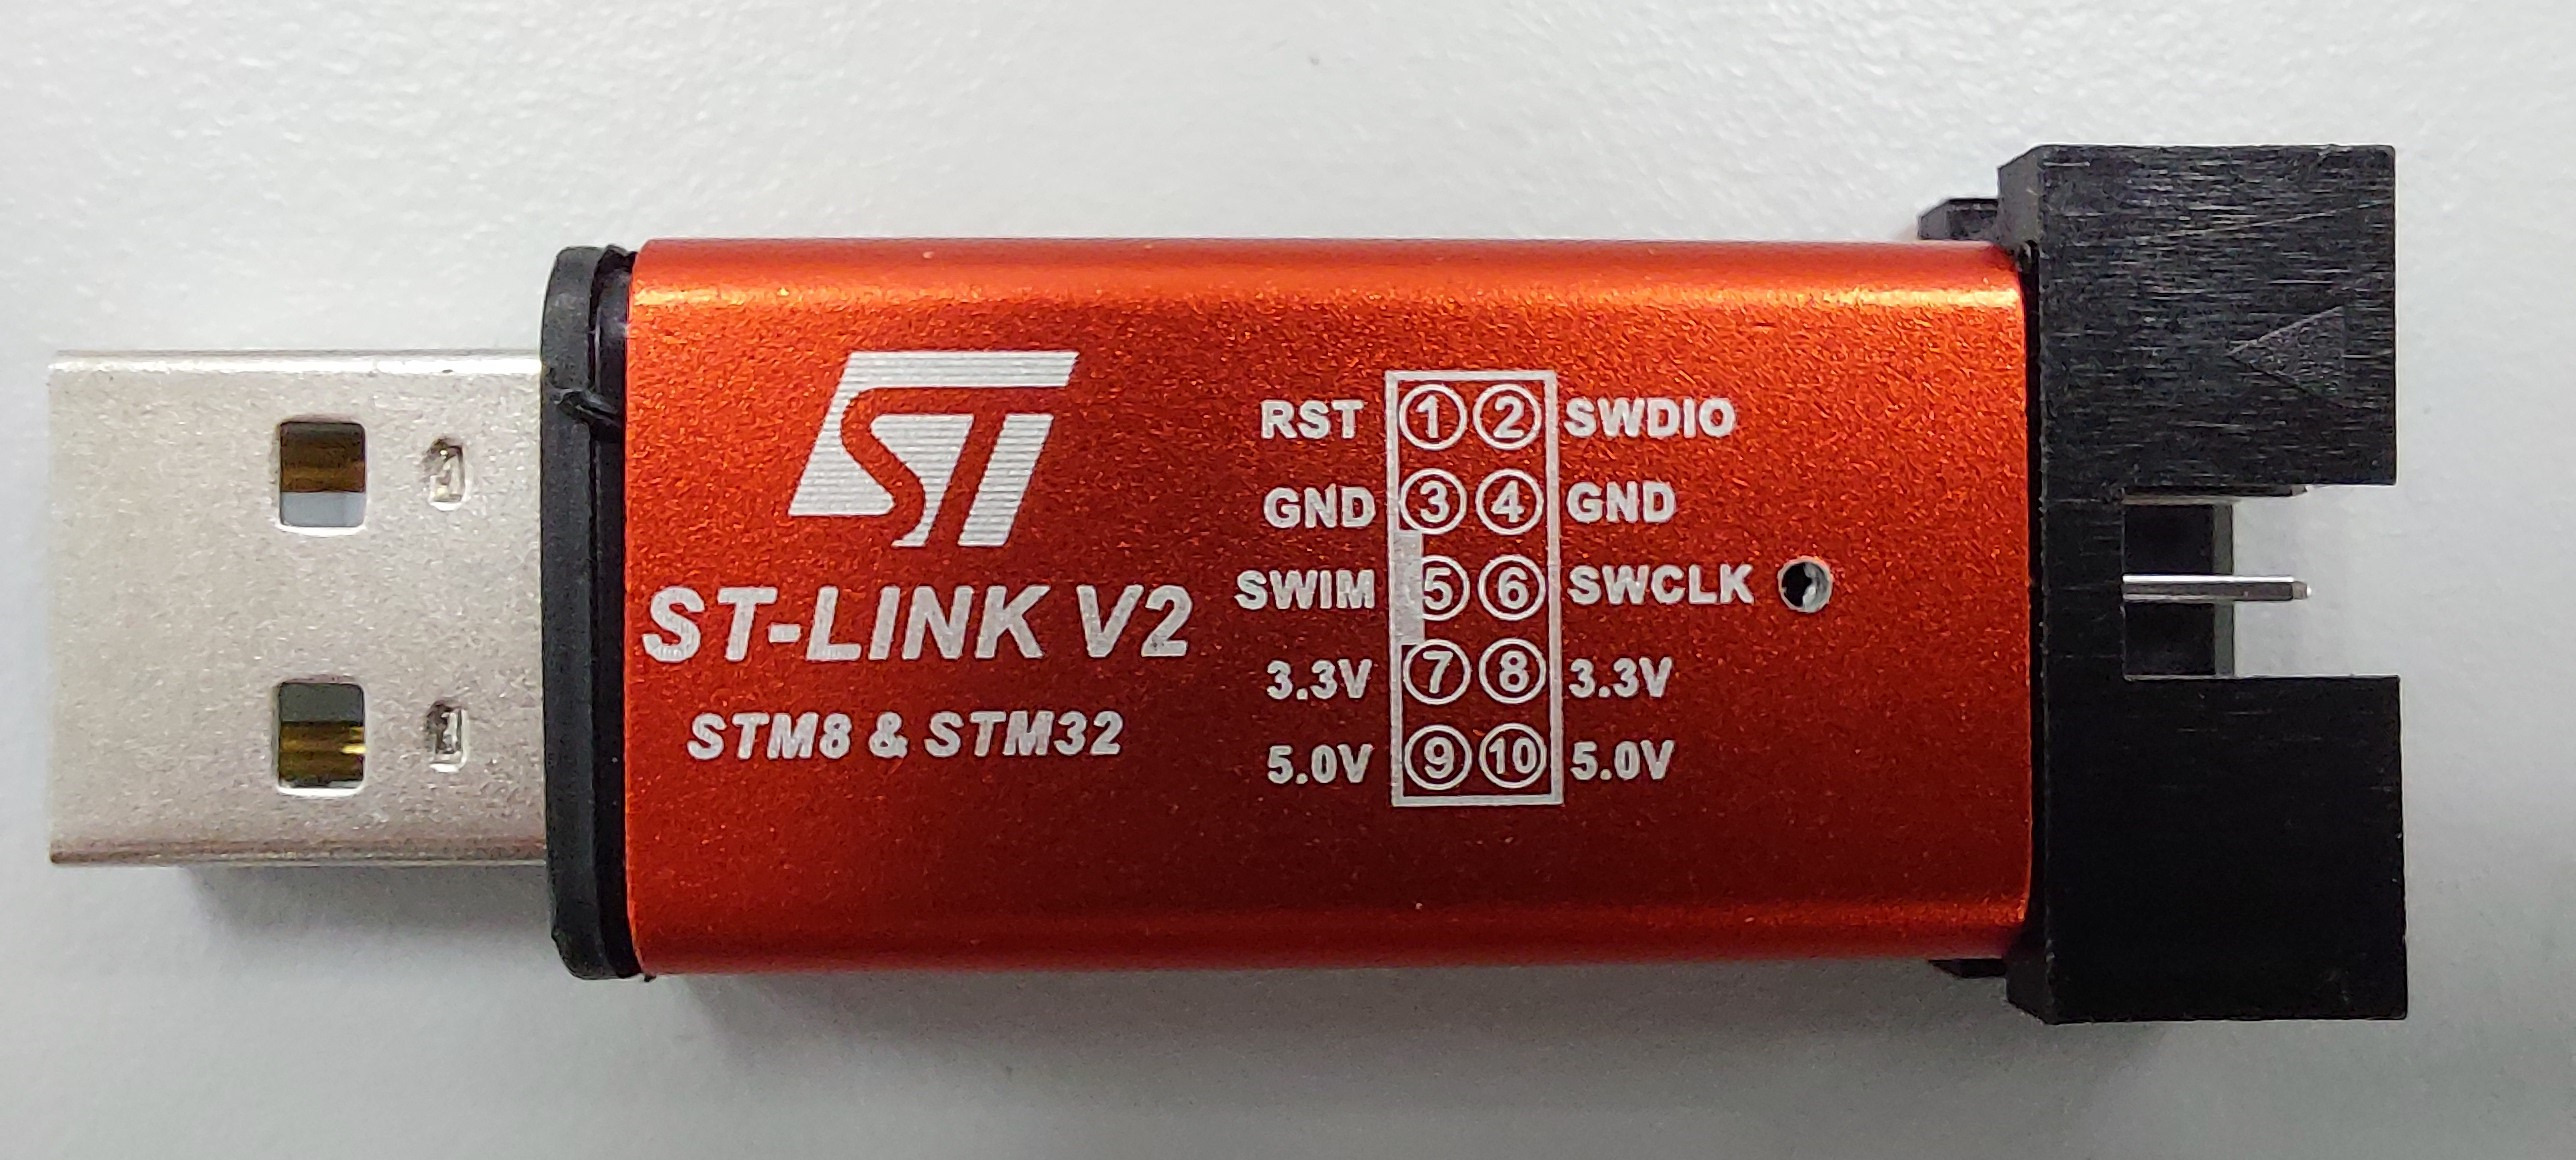
\includegraphics[width=4in]{figs/stlink.jpg}
  \caption{A Chinese copy of a ST-link programmer.  Unfortunately, the
    copiers are not consistent with the pinout!}
  \label{fig:stlink}
\end{figure}


The SAM4S is programmed and debugged using the serial wire debug (SWD)
protocol.  This requires an ST-link programmer that you can get from
Scott Lloyd in the SMT lab.

You will need to make your own cable to connect the ST-link programmer
to your board.  To reduce confusion, for a grey ribbon cable, align
the red stripe with the small arrow denoting pin 1 on the
connector. For a rainbow ribbon cable, connect the brown wire to pin
1.

Note, there are two variants of the ST-link programmer with
\textbf{different pinouts}, so you may need to customise your
programming cable.

The ST-programmer provides 3.3\,V to run the SAM4S during programming.
To reduce confusion, I suggest you disconnect the cable when running
off a battery or bench power supply.  Otherwise, recycling the power
will not reset the SAM4S since the ST-programmer will maintain the
3.3\, power supply.


\section{Connecting with OpenOCD}
\label{openocd}

\begin{figure}
\input{figs/openocd.schtex}
\caption{How OpenOCD interacts with the debugger and the SAM4S.}
\label{fig:openocd diagram}
\end{figure}


\program{OpenOCD} is used to program the SAM4S, see \reffig{openocd
  diagram}.

For this assignment, we use a \hyperref[ST-link]{ST-link programmer}
to connect to the SAM4S using serial wire debug (SWD). This connects
to your board with a 10-wire ribbon cable and an IDC connector.

\begin{enumerate}
\item
  Before you start, disconnect the battery and other cables from your
  PCB.

\item
  Connect a 10-wire ribbon cable from the \hyperref[ST-link]{ST-link
    programmer} to the programming header on your PCB.  This will
  provide 3.3\,V to your board so your green power LED should light.

\item
  \textbf{Command line:} open a new terminal window, e.g., bash and
  start \program{OpenOCD}:
  \begin{minted}{bash}
  $ cd wacky-racers
  $ openocd -f src/mat91lib/sam4s/scripts/sam4s_stlink.cfg
  \end{minted}
  (If using Windows, make sure you have set up the toolchain environment
  by running
  \file{C:\textbackslash{}ence461\textbackslash{}ence461-path}. See
  Section~\ref{esl-windows/command-line}.)

  \textbf{VS Code:} run the \code{Launch OpenOCD} task from the
  build menu (\code{Ctrl+Shift+B}) with
  \wfile{test-apps/ledflash1/ledflash1.c} open in the editor.
\end{enumerate}

All going well, the last line output from \program{OpenOCD} should be:
\begin{verbatim}
Info : sam4.cpu: hardware has 6 breakpoints, 4 watchpoints
\end{verbatim}

Congrats if you get this! It means you have correctly soldered your
SAM4S. If not, do not despair and do not remove your SAM4S. Instead,
see \protect\hyperref[sam4s-not-detected-by-openocd]{SAM4S not
  detected by OpenOCD}.

You can now stop OpenOCD with ctrl-c.  From now on you should not need
to manually run OpenOCD like this; it will be automatically run in the
background when you program or debug the SAM4S.


\section{LED flash program}
\label{led-flash-program}

For your first program, use
\wfile{test-apps/ledflash1/ledflash1.c}. The macro \code{LED_STATUS_PIO}
needs to be defined in \file{target.h} (see
\protect\hyperref[configuration]{configuration}).

\inputminted{C}{../../src/test-apps/ledflash1/ledflash1.c}


\section{Configuration}
\label{configuration}

Each board has different PIO definitions and requires its own
configuration information. The \wfile{boards} directory contains a
configuration for the hat and one for the racer board.  \textbf{You
must edit these to customise your board.}  Each configuration
directory contains three files:

\begin{itemize}
\item
  \file{board.mk} is a makefile fragment that specifies the MCU model,
  default optimisation level, etc.
\item
  \file{target.h} is a C header file that defines the PIO pins and
  clock speeds for the target system.
\item
  \file{config.h} is a C header file that wraps target.h.  Its purpose
  is for porting to different compilers.
\end{itemize}

\textbf{You will need to edit the target.h file for your board} and set
the definitions appropriate for your hardware. Here's an excerpt from
\file{target.h} for a hat board:

\begin{minted}{C}
/* ADC  */
#define ADC_BATTERY PB3_PIO

/* LEDs  */
#define LED_STATUS_PIO PA20_PIO
#define LED_ERROR__PIO PA23_PIO
\end{minted}


\section{Compilation}
\label{compilation}

Due to the many files required, compilation is performed using
makefiles. You can compile the programs using either the command line or
VS Code.

\begin{description}
  \item[Command line:] the demo test programs are generic and you need
  to specify which board you are compiling them for. The board
  configuration file can be chosen dynamically by defining the
  environment variable \code{BOARD} to either \code{hat} or
  \code{racer}. For example:
  %
  \begin{minted}{bash}
  $ cd src/test-apps/ledflash1
  $ make BOARD=racer
  \end{minted}

  To avoid having to specify the environment variable \code{BOARD}, you
  can define it for the rest of your session using:
  %
  \begin{minted}{bash}
  $ export BOARD=racer
  \end{minted}
  %
  and then just use:
  %
  \begin{minted}{bash}
  $ make
  \end{minted}
  (If using Windows Command Prompt, replace \code{export} with \code{set}.)

  \item[VS Code:] make sure you have selected the correct target board
  (\code{hat} or \code{racer}) in the bottom right corner (see
  Section~\ref{vs-code}). Then with \code{ledflash1.c} open in the editor,
  press \code{Ctrl+Shift+B} and run the \code{Build} task.
\end{description}

If all goes well, you should see at the end:
\begin{verbatim}
   text      data     bss     dec     hex filename
  17184        28     892   18104    46b8 build/app.elf
\end{verbatim}
(Note the numbers may be slightly different due to your version of the
compiler.  This is fine.)


\section{Booting from flash memory}
\label{booting-from-flash-memory}

If the SAM4S has never been programmed, on reset it runs a bootloader
program stored in ROM.  To run your application in flash memory, you
need to set a special bit also stored in flash memory.

\begin{description}
  \item[Command line:] from the test app directory:
  \begin{minted}{bash}
  $ make BOARD=[board] bootflash
  \end{minted}

  \item[VS Code:] with the test app open in the editor, press
  \code{Ctrl+Shift+B} and run the \code{Bootflash} task.
\end{description}

Unless you force a complete erasure of the SAM4S flash memory by
connecting the \pin{ERASE} pin to 3.3\,V, you will not need to repeat
this command.

\section{Programming}\label{programming}

\begin{description}
  \item[Command line:] from the test app directory, run:
  \begin{minted}{bash}
  $ make BOARD=[board] program
  \end{minted}

  \item[VS Code:] with the test app open in the editor, press
  \code{Ctrl+Shift+B} and run the \code{Program} task.
\end{description}

When this finishes, one of your LEDs should flash. If so, congrats! If
not, see \protect\hyperref[troubleshooting]{troubleshooting}.


\section{Makefiles}

Compilation is performed using makefiles, since each application
requires many files.  Rather than having large makefiles, a heirarchy
of makefile fragments is employed.  Dependencies are automatically
generated (so not all the files have to be recompiled each time).

A board description can be selected with the \code{BOARD} environment
variable.  This can be defined for each command, for example,
%
\begin{minted}{bash}
$ make BOARD=racer program
\end{minted}


Alternatively, this can be defined for a session:
%
\begin{minted}{bash}
$ export BOARD=racer
$ make program
\end{minted}

You can also explicitly set \code{BOARD} inside the Makefile (e.g., if
you have a board-specific program):
%
\begin{minted}{makefile}
BOARD = racer
\end{minted}

Each of the makefiles has the following phony targets, each of which
corresponds to a task in the VS Code task menu (\code{Ctrl+Shift+B}):

\begin{tabular}{lll}
  \toprule
  Make target & VS Code task & Description \\
  \midrule
  \code{all}     & \textit{Build}                & Compile the application \\
  \code{program} & \textit{Program}              & Compile the application and download to the MCU \\
  \code{debug}   & \textit{Debug (command line)} & Start the debugger GDB \\
  \code{clean}   & \textit{Clean}                & Delete the executable, object files, and dependency files \\
  \code{openocd} & \textit{Launch OpenOCD}       & Launch OpenOCD and attempt to connect to target \\
  \bottomrule
\end{tabular}
